\documentclass[11pt,a4paper]{report}
\usepackage[textwidth=37em,vmargin=30mm]{geometry}
\usepackage{calc,xunicode,amsmath,amssymb,paralist,enumitem,tabu,booktabs,datetime2,xeCJK,xeCJKfntef,listings}
\usepackage{tocloft,fancyhdr,tcolorbox,xcolor,graphicx,eso-pic,xltxtra,xelatexemoji}

\newcommand{\envyear}[0]{2025}
\newcommand{\envdatestr}[0]{2025-06-19}
\newcommand{\envfinaldir}[0]{webdb/2025/20250619/final}

\usepackage[hidelinks]{hyperref}
\hypersetup{
    colorlinks=false,
    pdfpagemode=FullScreen,
    pdftitle={Web Digest - \envdatestr}
}

\setlength{\cftbeforechapskip}{10pt}
\renewcommand{\cftchapfont}{\rmfamily\bfseries\large\raggedright}
\setlength{\cftbeforesecskip}{2pt}
\renewcommand{\cftsecfont}{\sffamily\small\raggedright}

\setdefaultleftmargin{2em}{2em}{1em}{1em}{1em}{1em}

\usepackage{xeCJK,xeCJKfntef}
\xeCJKsetup{PunctStyle=plain,RubberPunctSkip=false,CJKglue=\strut\hskip 0pt plus 0.1em minus 0.05em,CJKecglue=\strut\hskip 0.22em plus 0.2em}
\XeTeXlinebreaklocale "zh"
\XeTeXlinebreakskip = 0pt


\setmainfont{Brygada 1918}
\setromanfont{Brygada 1918}
\setsansfont{IBM Plex Sans}
\setmonofont{JetBrains Mono NL}
\setCJKmainfont{Noto Serif CJK SC}
\setCJKromanfont{Noto Serif CJK SC}
\setCJKsansfont{Noto Sans CJK SC}
\setCJKmonofont{Noto Sans CJK SC}

\setlength{\parindent}{0pt}
\setlength{\parskip}{8pt}
\linespread{1.15}

\lstset{
	basicstyle=\ttfamily\footnotesize,
	numbersep=5pt,
	backgroundcolor=\color{black!5},
	showspaces=false,
	showstringspaces=false,
	showtabs=false,
	tabsize=2,
	captionpos=b,
	breaklines=true,
	breakatwhitespace=true,
	breakautoindent=true,
	linewidth=\textwidth
}






\newcommand{\coverpic}[2]{
    % argv: itemurl, authorname
    Cover photo by #2~~(\href{#1}{#1})
}
\newcommand{\makeheader}[0]{
    \begin{titlepage}
        % \newgeometry{hmargin=15mm,tmargin=21mm,bmargin=12mm}
        \begin{center}
            
            \rmfamily\scshape
            \fontspec{BaskervilleF}
            \fontspec{Old Standard}
            \fontsize{59pt}{70pt}\selectfont
            WEB\hfill DIGEST
            
            \vfill
            % \vskip 30pt
            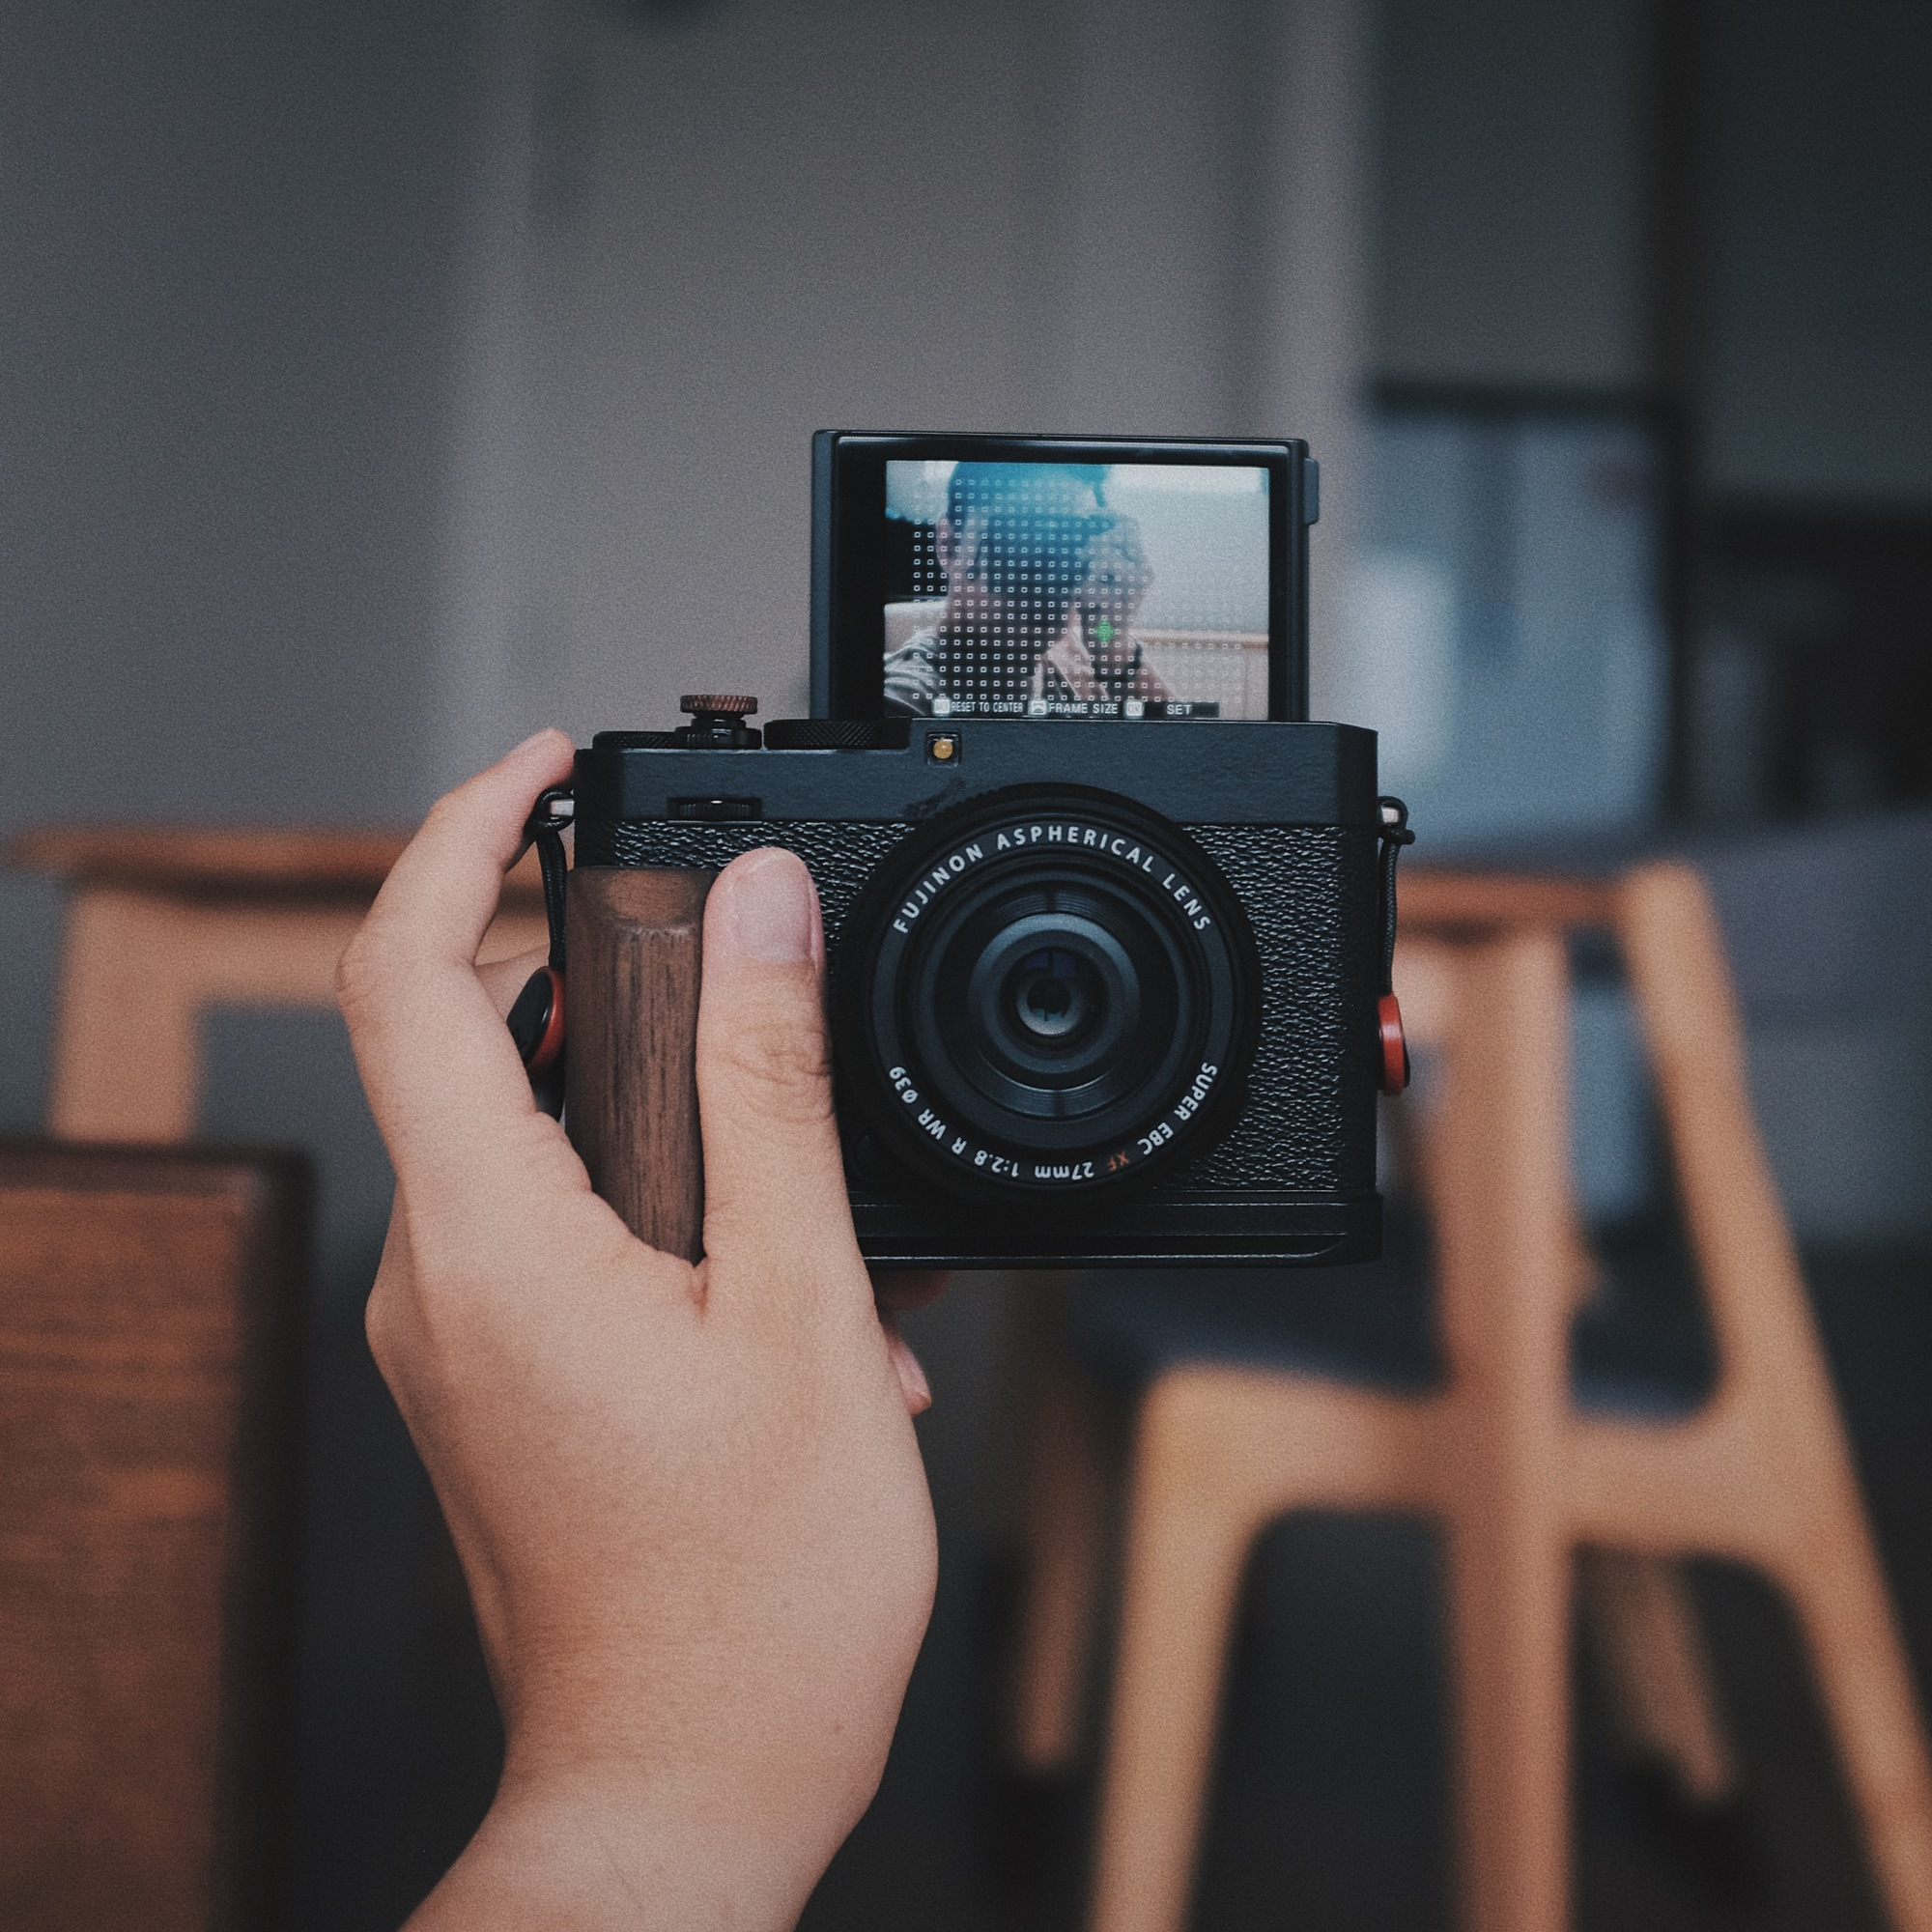
\includegraphics[width=\linewidth]{\envfinaldir/coverpic-prod.jpg}\par
            % \vskip 30pt
            \vfill

            \normalsize\rmfamily\scshape
            \copyright{} The Web Digest Project \hfill\large \envdatestr
        \end{center}
    \end{titlepage}
    % \restoregeometry
}
\newcommand{\simplehref}[1]{%
    \textcolor{blue!80!green}{\href{#1}{#1}}%
}
\renewcommand{\contentsname}{\center\Huge\sffamily\bfseries Contents\par\vskip 20pt}
\newcounter{ipartcounter}
\setcounter{ipartcounter}{0}
\newcommand{\ipart}[1]{
    % \vskip 20pt
    \clearpage
    \stepcounter{ipartcounter}
    \phantomsection
    \addcontentsline{toc}{chapter}{#1}
    % \begin{center}
    %     \Huge
    %     \sffamily\bfseries
    %     #1
    % \end{center}
    % \vskip 20pt plus 7pt
}
\newcounter{ichaptercounter}
\setcounter{ichaptercounter}{0}
\newcommand{\ichapter}[1]{
    % \vskip 20pt
    \clearpage
    \stepcounter{ichaptercounter}
    \phantomsection
    \addcontentsline{toc}{section}{\numberline{\arabic{ichaptercounter}}#1}
    \begin{center}
        \Huge
        \sffamily\bfseries
        #1
    \end{center}
    \vskip 20pt plus 7pt
}
\newcommand{\entrytitlefont}[1]{\subsection*{\raggedright\Large\sffamily\bfseries#1}}
\newcommand{\entryitemGeneric}[2]{
    % argv: title, url
    \parbox{\linewidth}{
        \entrytitlefont{#1}\par\vskip 5pt
        \footnotesize\ttfamily\mdseries
        \simplehref{#2}
    }\vskip 11pt plus 11pt minus 1pt
}
\newcommand{\entryitemGithub}[3]{
    % argv: title, url, desc
    \parbox{\linewidth}{
        \entrytitlefont{#1}\par\vskip 5pt
        \footnotesize\ttfamily\mdseries
        \simplehref{#2}\par\vskip 5pt
        \small\rmfamily\mdseries#3
    }\vskip 11pt plus 11pt minus 1pt
}
\newcommand{\entryitemAp}[3]{
    % argv: title, url, desc
    \parbox{\linewidth}{
        \entrytitlefont{#1}\par\vskip 5pt
        \footnotesize\ttfamily\mdseries
        \simplehref{#2}\par\vskip 5pt
        \small\rmfamily\mdseries#3
    }\vskip 11pt plus 11pt minus 1pt
}
\newcommand{\entryitemHackernews}[3]{
    % argv: title, hnurl, rawurl
    % \parbox{\linewidth}{
    %     \entrytitlefont{#1}\par\vskip 5pt
    %     \footnotesize\ttfamily\mdseries
    %     \simplehref{#3}\par
    %     \textcolor{black!50}{\href{#2}{#2}}
    % }\vskip 11pt plus 11pt minus 1pt
    \begin{minipage}{\linewidth}
            \entrytitlefont{#1}\par\vskip 5pt
            \footnotesize\ttfamily\mdseries
            \simplehref{#3}\par
            \textcolor{black!50}{\href{#2}{#2}}
    \end{minipage}\par\vskip 11pt plus 11pt minus 1pt
}







\begin{document}

\makeheader

\tableofcontents\clearpage




\ipart{Developers}
\ichapter{Hacker News}
\entryitemTwoLinks{Andrej Karpathy's YC AI SUS talk on the future of the industry}{https://news.ycombinator.com/item?id=44311509}{https://www.donnamagi.com/articles/karpathy-yc-talk}

\entryitemTwoLinks{The unreasonable effectiveness of fuzzing for porting programs}{https://news.ycombinator.com/item?id=44311241}{https://rjp.io/blog/2025-06-17-unreasonable-effectiveness-of-fuzzing}

\entryitemTwoLinks{Writing documentation for AI: best practices}{https://news.ycombinator.com/item?id=44311217}{https://docs.kapa.ai/improving/writing-best-practices}

\entryitemTwoLinks{My iPhone 8 Refuses to Die: Now It's a Solar-Powered Vision OCR Server}{https://news.ycombinator.com/item?id=44310944}{https://terminalbytes.com/iphone-8-solar-powered-vision-ocr-server/}

\entryitemTwoLinks{Framework Laptop 12 review}{https://news.ycombinator.com/item?id=44310583}{https://arstechnica.com/gadgets/2025/06/framework-laptop-12-review-im-excited-to-see-what-the-2nd-generation-looks-like/}

\entryitemTwoLinks{Homomorphically Encrypting CRDTs}{https://news.ycombinator.com/item?id=44309520}{https://jakelazaroff.com/words/homomorphically-encrypted-crdts/}

\entryitemTwoLinks{Show HN: Workout.cool – Open-source fitness coaching platform}{https://news.ycombinator.com/item?id=44309320}{https://github.com/Snouzy/workout-cool}

\entryitemTwoLinks{Is there a half-life for the success rates of AI agents?}{https://news.ycombinator.com/item?id=44308711}{https://www.tobyord.com/writing/half-life}

\entryitemTwoLinks{Terpstra Keyboard}{https://news.ycombinator.com/item?id=44308558}{http://terpstrakeyboard.com/web-app/keys.htm}

\entryitemTwoLinks{I counted all of the yurts in Mongolia using machine learning}{https://news.ycombinator.com/item?id=44307629}{https://monroeclinton.com/counting-all-yurts-in-mongolia/}

\entryitemTwoLinks{MiniMax-M1 open-weight, large-scale hybrid-attention reasoning model}{https://news.ycombinator.com/item?id=44307290}{https://github.com/MiniMax-AI/MiniMax-M1}

\entryitemTwoLinks{Your Brain on ChatGPT}{https://news.ycombinator.com/item?id=44307257}{https://www.media.mit.edu/projects/your-brain-on-chatgpt/overview/}

\entryitemTwoLinks{Scrappy – Make little apps for you and your friends}{https://news.ycombinator.com/item?id=44306859}{https://pontus.granstrom.me/scrappy/}

\entryitemTwoLinks{Locally hosting an internet-connected server}{https://news.ycombinator.com/item?id=44306792}{https://mjg59.dreamwidth.org/72095.html}

\entryitemTwoLinks{Show HN: Lstr – A modern, interactive tree command written in Rust}{https://news.ycombinator.com/item?id=44306041}{https://github.com/bgreenwell/lstr}

\entryitemTwoLinks{The Grug Brained Developer (2022)}{https://news.ycombinator.com/item?id=44303542}{https://grugbrain.dev/}

\entryitemTwoLinks{Bzip2 crate switches from C to 100\% Rust}{https://news.ycombinator.com/item?id=44303361}{https://trifectatech.org/blog/bzip2-crate-switches-from-c-to-rust/}

\entryitemTwoLinks{What Google Translate can tell us about vibecoding}{https://news.ycombinator.com/item?id=44302870}{https://ingrids.space/posts/what-google-translate-can-tell-us-about-vibecoding/}

\entryitemTwoLinks{LLMs pose an interesting problem for DSL designers}{https://news.ycombinator.com/item?id=44302797}{https://kirancodes.me/posts/log-lang-design-llms.html}

\entryitemTwoLinks{Iran asks its people to delete WhatsApp from their devices}{https://news.ycombinator.com/item?id=44302752}{https://apnews.com/article/iran-whatsapp-meta-israel-d9e6fe43280123c9963802e6f10ac8d1}


\ipart{Developers~~~~(zh-Hans)}
\ichapter{Solidot}
\entryitemGeneric{\hskip 0pt{}微生物被发现有类似病毒的特征}{https://www.solidot.org/story?sid=81593}

\entryitemGeneric{\hskip 0pt{}微软报告晚上八点后开会的次数在增加}{https://www.solidot.org/story?sid=81592}

\entryitemGeneric{\hskip 0pt{}Netflix 纪录片揭露 OceanGate 泰坦号潜艇事故的更多细节}{https://www.solidot.org/story?sid=81591}

\entryitemGeneric{\hskip 0pt{}伊朗禁止官员使用联网设备}{https://www.solidot.org/story?sid=81590}

\entryitemGeneric{\hskip 0pt{}生活在受微塑料污染的海边可能增加心血管代谢疾病风险 }{https://www.solidot.org/story?sid=81589}

\entryitemGeneric{\hskip 0pt{}使用大模型如何影响你的大脑}{https://www.solidot.org/story?sid=81588}

\entryitemGeneric{\hskip 0pt{}AMD 宣布 CDNA 4 架构}{https://www.solidot.org/story?sid=81587}

\entryitemGeneric{\hskip 0pt{}本田成功测试可重复使用火箭}{https://www.solidot.org/story?sid=81586}

\entryitemGeneric{\hskip 0pt{}为什么中国拥抱开源?}{https://www.solidot.org/story?sid=81585}

\entryitemGeneric{\hskip 0pt{}特朗普第三次给予 TikTok 90 天宽限期}{https://www.solidot.org/story?sid=81584}

\entryitemGeneric{\hskip 0pt{}伊朗计划全面断网}{https://www.solidot.org/story?sid=81583}

\entryitemGeneric{\hskip 0pt{}科学家创造出一种致命真菌去对抗蚊子}{https://www.solidot.org/story?sid=81582}

\entryitemGeneric{\hskip 0pt{}研究人员创造出第一种完全可验证的真随机数生成器}{https://www.solidot.org/story?sid=81581}

\entryitemGeneric{\hskip 0pt{}KDE Plasma 6.4 释出}{https://www.solidot.org/story?sid=81580}

\entryitemGeneric{\hskip 0pt{}特朗普集团宣布 499 美元智能手机}{https://www.solidot.org/story?sid=81579}

\entryitemGeneric{\hskip 0pt{}美国最主要的新闻来源如今是社交媒体}{https://www.solidot.org/story?sid=81578}

\entryitemGeneric{\hskip 0pt{}英特尔将裁减 15\%-20\% 的芯片工厂员工}{https://www.solidot.org/story?sid=81577}

\entryitemGeneric{\hskip 0pt{}OpenAI 和微软之间的紧张关系加剧 }{https://www.solidot.org/story?sid=81576}

\entryitemGeneric{\hskip 0pt{}Nexus Mods 创始人卸任}{https://www.solidot.org/story?sid=81575}

\entryitemGeneric{\hskip 0pt{}大部分重子物质藏身于星际之间}{https://www.solidot.org/story?sid=81574}\ichapter{V2EX}
\entryitemGeneric{\hskip 0pt{}[Windows] 发现 Windows 10/11 LTSC 安装 Microsoft Store 其实如此简单,只用一行简短的命令}{https://www.v2ex.com/t/1139564}

\entryitemGeneric{\hskip 0pt{}[问与答] 请教有没有比较靠谱的自动为视频添加双语字幕的方案?}{https://www.v2ex.com/t/1139562}

\entryitemGeneric{\hskip 0pt{}[分享发现] 记一次诡异的经历:更换 CPU 之后 Chrome 打不开了}{https://www.v2ex.com/t/1139561}

\entryitemGeneric{\hskip 0pt{}[硬件] 400 块钱捡了一套家庭影院...}{https://www.v2ex.com/t/1139560}

\entryitemGeneric{\hskip 0pt{}[分享发现] Seo 工具使用与流量数据观察实践 上}{https://www.v2ex.com/t/1139559}

\entryitemGeneric{\hskip 0pt{}[生活] 买了个手机,却高兴不起来}{https://www.v2ex.com/t/1139558}

\entryitemGeneric{\hskip 0pt{}[分享创造] ExpDeals 5.0 更新,我又把 Priceline 给破了. 全新的 Map View/Zone 比较}{https://www.v2ex.com/t/1139556}

\entryitemGeneric{\hskip 0pt{}[程序员] 你们用的哪种 ~ 操作浏览器的 MCP 方案}{https://www.v2ex.com/t/1139555}

\entryitemGeneric{\hskip 0pt{}[VXNA] 申请收录个人博客: Frytea's Blog}{https://www.v2ex.com/t/1139554}

\entryitemGeneric{\hskip 0pt{}[Windows] Windows 远程连接暴露在公网被疯狂爆破}{https://www.v2ex.com/t/1139552}

\entryitemGeneric{\hskip 0pt{}[随想] 原以为好看的电影有那么多供任意挑选}{https://www.v2ex.com/t/1139551}

\entryitemGeneric{\hskip 0pt{}[分享发现] Microsoft PowerToys,一款深度 windows 者的实用工具}{https://www.v2ex.com/t/1139548}

\entryitemGeneric{\hskip 0pt{}[分享创造] 瞬间提升 Umami 数据直观性的开源 Dashboard}{https://www.v2ex.com/t/1139547}

\entryitemGeneric{\hskip 0pt{}[摄影] 今天晚上竟然用无人机拍到了闪电!}{https://www.v2ex.com/t/1139546}

\entryitemGeneric{\hskip 0pt{}[职场话题] 毕业即失业,打算自学 RISC-V,大家有什么建议?}{https://www.v2ex.com/t/1139545}

\entryitemGeneric{\hskip 0pt{}[Apple] ios16.6 配对了 watch11.4,目前就是蜂窝无法开通,一直显示连接失败,求高手帮助}{https://www.v2ex.com/t/1139544}

\entryitemGeneric{\hskip 0pt{}[Telegram] 关于 telegram appid 代办挣了几十块}{https://www.v2ex.com/t/1139543}

\entryitemGeneric{\hskip 0pt{}[Podcast] [分享] 我把全球优质播客翻译成了超自然的中文声音,连我爸都听懂了}{https://www.v2ex.com/t/1139542}

\entryitemGeneric{\hskip 0pt{}[宽带症候群] 如何获取宽带密码}{https://www.v2ex.com/t/1139541}

\entryitemGeneric{\hskip 0pt{}[深圳] 求租|深圳南山区}{https://www.v2ex.com/t/1139540}

\entryitemGeneric{\hskip 0pt{}[程序员] 购买 AI 助手最廉价的方案}{https://www.v2ex.com/t/1139538}

\entryitemGeneric{\hskip 0pt{}[问与答] 前端大神进来下,有没有这样的前端开源框架?}{https://www.v2ex.com/t/1139536}

\entryitemGeneric{\hskip 0pt{}[问与答] 假设一个文件夹里有大量图片,有什么 ai 工具可以自动分析图片,然后根据图片的色系和内容来重新命名图片?}{https://www.v2ex.com/t/1139533}

\entryitemGeneric{\hskip 0pt{}[全球工单系统] 又接到腾讯游戏骚扰电话了}{https://www.v2ex.com/t/1139532}

\entryitemGeneric{\hskip 0pt{}[职场话题] 成都求跳槽建议:现职被动降薪,新 offer 二选一}{https://www.v2ex.com/t/1139531}

\entryitemGeneric{\hskip 0pt{}[Apple] 求推荐好用的 mac mini 键盘}{https://www.v2ex.com/t/1139530}

\entryitemGeneric{\hskip 0pt{}[程序员] trae 使用 Claude 3.5 Sonnet 充当 Claude 4 Sonnet}{https://www.v2ex.com/t/1139529}

\entryitemGeneric{\hskip 0pt{}[问与答] 两台 Mac 共用一台显示器和一套键鼠的最佳方案是什么?}{https://www.v2ex.com/t/1139528}

\entryitemGeneric{\hskip 0pt{}[macOS] Mac mini(m4)最新版系统(15.5),安装下载的 quark/chrome/edge/微信输入法都失败}{https://www.v2ex.com/t/1139527}

\entryitemGeneric{\hskip 0pt{}[生活] 有人了解住院陪护的价格和服务质量吗}{https://www.v2ex.com/t/1139525}

\entryitemGeneric{\hskip 0pt{}[V2EX 站点状态] 20250618 - OTP 输入有时候会失效的问题似乎是修好了}{https://www.v2ex.com/t/1139524}

\entryitemGeneric{\hskip 0pt{}[程序员] 今天 iOS 有什么关于 SSL 的更新吗?还是有什么我不知道的机制}{https://www.v2ex.com/t/1139523}

\entryitemGeneric{\hskip 0pt{}[程序员] 10 年了,你还在用 2005 年的 Git 命令吗?}{https://www.v2ex.com/t/1139522}

\entryitemGeneric{\hskip 0pt{}[OpenAI] 大家有没有晚上 GPT 卡顿的情况}{https://www.v2ex.com/t/1139521}

\entryitemGeneric{\hskip 0pt{}[OpenAI] 尝试写 Prompt 模拟了下站内老哥的 GPT 英汉字典}{https://www.v2ex.com/t/1139520}

\entryitemGeneric{\hskip 0pt{}[问与答] frp 内网穿透到本地 mac 上的 wordpress 网站,无法访问}{https://www.v2ex.com/t/1139518}

\entryitemGeneric{\hskip 0pt{}[微信] +852 可以看到+86 用户的正在输入状态了}{https://www.v2ex.com/t/1139517}

\entryitemGeneric{\hskip 0pt{}[职场话题] 去面试,上去先给我一张表,让填各种信息,小学到高中的经历等等,我直接走了,大家会填吗?让填这个是什么目的呢?}{https://www.v2ex.com/t/1139516}

\entryitemGeneric{\hskip 0pt{}[分享创造] [开源] 看来是找不到工作了,那就继续做 Ai 小说写作平台吧,更新了第二个版本}{https://www.v2ex.com/t/1139515}

\entryitemGeneric{\hskip 0pt{}[汽车] 哪个车企的车机系统比较开放?}{https://www.v2ex.com/t/1139513}

\entryitemGeneric{\hskip 0pt{}[分享发现] 消息称三大运营商将于今年下半年全面重启 eSIM}{https://www.v2ex.com/t/1139512}

\entryitemGeneric{\hskip 0pt{}[宽带症候群] 奶昔的 Premium 如何?}{https://www.v2ex.com/t/1139511}

\entryitemGeneric{\hskip 0pt{}[问与答] 提问:虚拟机装腾讯那个 IOA 代理的问题}{https://www.v2ex.com/t/1139510}

\entryitemGeneric{\hskip 0pt{}[职场话题] ebay 的外包咋样啊,双休不加班}{https://www.v2ex.com/t/1139509}

\entryitemGeneric{\hskip 0pt{}[推广] 阿里云新用户折上折 3 折,可以续费, 59 元 2 年 2h2g 服务器}{https://www.v2ex.com/t/1139508}

\entryitemGeneric{\hskip 0pt{}[宽带症候群] 请教一个移动到香港带宽}{https://www.v2ex.com/t/1139506}

\entryitemGeneric{\hskip 0pt{}[问与答] 请问大家,油烟机怎么选?}{https://www.v2ex.com/t/1139504}

\entryitemGeneric{\hskip 0pt{}[分享创造] 公众号排版太麻烦?分享一款极简美学的微信 Markdown 编辑器,同时内置了三款热门主题!复制粘贴就能用!}{https://www.v2ex.com/t/1139503}

\entryitemGeneric{\hskip 0pt{}[程序员] 很奇怪,为什么使用 Rust 开发的软件,作者喜欢把 Rust 作为宣传点之一}{https://www.v2ex.com/t/1139502}

\entryitemGeneric{\hskip 0pt{}[V2EX] 啊这是我没有想到的}{https://www.v2ex.com/t/1139501}


\ipart{Generic News}
\ichapter{联合早报}
\entryitemWithDescription{杨丹旭:关税战中找定力}{https://www.zaobao.com/news/china/story20250617-6814940}{中美伦敦经贸磋商后,美国媒体彭博社发表了一篇评论文章,概括中美对待这场贸易争端截然不同的两种思维:美国领导人急于出成果,而中国领导人专注打长线战。 评论指出,中美伦敦经贸磋商后,美国总统特朗普对谈判结果大加赞赏,不仅在社交媒体上宣布,已与中国达成``协议'',来自中国的关键磁铁将恢复供应,美国也承诺会放宽对中国学生的签证限制……}

\entryitemWithDescription{中国5月消费显著回升达6.4\%成经济亮点 工业与房地产仍负重前行}{https://www.zaobao.com/news/china/story20250616-6807120}{在中美贸易战阴霾下,中国5月消费创下6.4\%的超预期增长,为一年半来最高增速,部分缓解了美国加征关税对中国增长的压力,但工业和房地产市场依然在负重前行。 中国官方表示,5月消费增长得益于多重利好因素叠加,包括``五一''\,``端午''假日消费、消费品以旧换新政策的带动,以及中国电商今年提早启动``618''大促等。分析预计北京将继续通过补贴政策刺激消费,并有可能出台新措施以稳定房地产市场……}

\entryitemWithDescription{福建舰下水三周年 中国官媒称三航母时代即将到来}{https://www.zaobao.com/news/china/story20250616-6811085}{(北京/香港综合讯)中国官媒透露,中国第三艘航母福建舰的海试工作正按计划稳步推进,海军三航母时代即将到来。有学者分析,福建舰服役后可直接压缩台军预警时间。 据央视新闻节目《军情时间到》上星期六(6月14日)报道,福建舰迎来下水三周年之际,相关建设和海事工作不断推进。福建舰入列后,将大幅提升中国海军近海防御和远海护卫作战的能力,中国海军也将正式进入三航母时代……}

\entryitemWithDescription{赖清德吁台美共同生产研发军备}{https://www.zaobao.com/news/china/story20250616-6811831}{(台北综合讯)台湾总统赖清德星期一(6月16日)接见到访的美国联邦众议员时表示,希望台美安全合作从军购迈向``共同生产、共同研发''伙伴关系……}

\entryitemWithDescription{夏宝龙据报星期三访港 将与八所大学高层闭门座谈}{https://www.zaobao.com/news/china/story20250616-6812113}{(香港综合讯)香港国安法实施五周年之际,中国国务院港澳事务办公室主任夏宝龙据报星期三(6月18日)起赴港调研五天。 香港《信报》星期一(16日)引述消息称,夏宝龙访港日期基本敲定在6月18日至22日,五天行程紧凑,除了出席星期六(21日)举办的``香港国安法公布实施五周年论坛''外,他还将到地方了解民情、与商界领袖座谈……}

\entryitemWithDescription{香港今年将提前发表《施政报告》 学者预计重点是发展经济}{https://www.zaobao.com/news/china/story20250616-6810243}{香港新一届立法会选举将在今年底举行,特区政府为此将首次提前在9月发表新一份《施政报告》。受访学者预计,由于香港经济不景气,今年《施政报告》除了继续加强国家安全领域的建设,也会着力提出发展经济的措施。 港府星期一(6月16日)宣布,行政长官李家超将在9月发表任内第四份《施政报告》,并从即日起展开公众咨询。期间,港府将举办逾40场咨询会,听取立法会议员、不同界别代表和公众对《施政报告》的意见和建议……}

\entryitemWithDescription{中国5月青年失业率连续三个月下降}{https://www.zaobao.com/news/china/story20250616-6804387}{(北京综合讯)中国国家统计局发言人付凌晖说,中国5月全国城镇调查失业率跌至5%,其中青年失业率连续三个月下降,但外部环境复杂变化冲击劳动力市场,使稳定就业仍面临一定压力。 中国国家统计局星期一(6月16日)公布的数据显示,5月全国城镇调查失业率较4月跌0.1个百分点。官方并未公布具体的青年失业率数据……}

\entryitemWithDescription{沈泽玮:中国网民看伊朗又菜又怂}{https://www.zaobao.com/news/china/story20250616-6782994}{以色列突袭伊朗,伊朗伊斯兰革命卫队总司令等多名高级指挥官和核科学家被一锅端。 以伊冲突在中国社交媒体平台上引来不少关注,让好些网民意外的是,伊朗防空系统形同虚设,被以色列和美国渗透如筛子,还浑然不知。 以色列背后的支持者是美国。中国、俄罗斯、伊朗大三角则被视为伙伴,中俄伊自2019年起就展开年度联合海上军演……}

\entryitemWithDescription{台湾将华为和中芯国际列入出口管制名单 两岸紧张或进一步加剧}{https://www.zaobao.com/news/china/story20250615-6782583}{中国大陆双航母同时现身西太平洋几天后,台湾在陆美贸易谈判拉锯之际,对华为和中芯国际等大陆高端晶片研发企业发布出口禁令。 受访学者认为,台湾此举一方面是配合美国,补上对大陆尖端晶片管制的缺口;另一方面也通过打压华为来表达对近期大陆对台一系列动作的不满,两岸紧张局势或进一步加剧……}

\entryitemWithDescription{北京故宫传漏水淋湿明代书画}{https://www.zaobao.com/news/china/story20250615-6782923}{(北京综合讯)中国首都北京突降暴雨,网传故宫博物院因此漏水,淋湿了明代书画。 综合极目新闻和中国青年网旗下短视频官微等报道,上星期六(6月14日),有网民在社交平台上分享视频并配文,称当天雷暴雨导致故宫午门漏雨。网民称在``乐林泉泉------中外园林文化展''展厅中,看到``豆大的雨滴滴在《东园图》卷上'',置于展柜中的``东''字左部疑似被雨滴淋湿……}

\entryitemWithDescription{中国歼-10实战击落法制战机后将在巴黎航展首秀}{https://www.zaobao.com/news/china/story20250615-6781912}{(北京讯)中国战斗机歼-10实战击落法制战机后,将在巴黎航展上首次亮相。 中国航空工业集团星期天(6月15日)在微信公众号公布,第55届巴黎航展将于6月16日至22日举行,该集团的参展阵容涵盖战斗机、无人机及民用飞机等,展现中国航空技术的建设成果。 在军机板块,展示机型将聚焦``20''家族,包括战机歼-20、歼-35A、歼-10CE、大型运输机运-20、直升机直-20及直-10ME……}

\entryitemWithDescription{中国恢复对美国出口军用稀土问题悬而未决 两国达成更全面贸易协议或遇阻}{https://www.zaobao.com/news/china/story20250615-6782240}{针对上周落幕的中美伦敦贸易谈判,路透社引述消息人士称,中国恢复对美国出口军用稀土问题依然悬而未决,美国也继续限制中国采购先进人工智能晶片,并考虑将8月10日到期的关税暂停期限,再延长90天。 受访学者分析,中美目前都不愿放弃对自己有利的牌,两国经贸博弈预计陷入漫长过程。 路透社星期天(6月15日)引述两名消息人士透露,中美在伦敦达成的贸易协议中,与国家安全相关的出口限制问题仍未解决……}

\entryitemWithDescription{随``达达的马蹄''远去 诗人郑愁予逝世}{https://www.zaobao.com/news/china/story20250615-6782446}{(台北综合讯)曾写下``我达达的马蹄是美丽的错误''的台湾著名诗人郑愁予,美国时间上星期五(6月13日)辞世,享耆寿91岁。 台湾《镜周刊》星期天(15日)向郑愁予亲友查证,确认他已于美国时间上星期五凌晨4时辞世。台湾诗人萧萧则引述郑愁予弟媳披露,郑愁予是因心脏衰竭去世。 《镜周刊》引述郑愁予的不具名亲友说:``大师带给台湾与华人世界多少浪漫与愁怅,愿他在天上与挚亲重逢,诗歌与音乐永远流传……}

\entryitemWithDescription{时隔一年举行人权对话 中欧再次交锋}{https://www.zaobao.com/news/china/story20250615-6782312}{(北京/布鲁塞尔综合讯)中国和欧盟举行年度人权对话并再度交锋。欧盟对中国基本自由持续恶化表示严重关切,中国则指欧盟国家存在民主自由倒退、侵犯难民移民权利、种族歧视等严重人权问题。 中国外交部国际司司长申博与欧盟对外行动署亚太总司副总司长帕姆帕罗尼上星期五(6月13日)在布鲁塞尔共同主持第40次中欧人权对话,这是两人继去年6月在重庆主持第39次对话后,时隔一年再会……}

\entryitemWithDescription{日企指世博会中国馆有上百万人民币工程费尚未支付}{https://www.zaobao.com/news/china/story20250615-6774913}{(大阪综合讯)参与大阪世博会中国馆建设的日本一家电气工程公司公开指,应收的3700万日元(32.9万新元,约184万元人民币)工程费尚未被支付。 据日本共同社中文网报道,这家来自日本神户市的电气工程公司,上星期五(6月13日)在大阪府政府大楼召开记者会,公司社长在会上作出上述指责。 报道称,这笔欠款源自去年11月前后至今年4月开幕前夕的追加工程费……}

\entryitemWithDescription{因美国征港口费中国船厂订单大减 今年首四个月跌三成}{https://www.zaobao.com/news/china/story20250615-6643855}{中国船厂今年以来新接订单同比大减,韩国船厂则逆势增长,反映在美国对中国船舶征收港口费政策的背景下,各国船东已开始调整订单,以规避地缘政治风险。 英国克拉克森研究公司(Clarkson Research)的数据显示,今年首四个月,中国新船订单达680万修正总吨(Compensated Gross Tonnage, CGT)。修正总吨指的是在船舶总吨基础上考虑进船舶复杂度而算出的船舶度量单位……}

\entryitemWithDescription{中国特稿:中国AI产业火爆赛道挤 广州新应用要弯道超车}{https://www.zaobao.com/news/china/story20250615-6713243}{借助人工智能(AI)工具,中国广州市一家汽车美容店的运营团队,半小时内生成100多条个性化视频,店员和顾客扫码转发这些视频后,店铺的新客源在那个星期同比增加50\%。 这家小型汽车美容店的三人团队,每天投入少量时间运营社交媒体账号,利用AI工具帮助产出内容,并进行投放与管理等,获客成本远低于传统模式。 这是广州创业公司 ``筷子科技``的一个销售案例……}

\entryitemWithDescription{国民党县市首长首度缺席海峡论坛 陆方赴台参加旅展被拒}{https://www.zaobao.com/news/china/story20250614-6760804}{(台北综合讯)两岸紧张关系持续影响双方交流,台湾在野党国民党的县市首长17年来首度缺席中国大陆主办的海峡论坛,大陆人士赴台参加两岸旅展的申请,也遭到台湾政府拒绝。 据《自由时报》报道,第十七届海峡论坛星期天(6月15日)起在福建举行。国民党籍县市首长首度缺席论坛,也没有派代表参加,国民党历来至少派出副主席层级参与,今年却仅由大陆事务部主任出席,层级明显下降……}

\entryitemWithDescription{中日就军机太平洋险距接触互相指责}{https://www.zaobao.com/news/china/story20250614-6760181}{(北京/东京综合讯)中国双航母编队首次同时现身西太平洋开展训练,一艘航母上起飞的中国战机与日本巡逻机近距离接触,引发两国互相指责。 日本国防部星期三(6月11日)通报,6月7日至8日,日本海上自卫队``P3C''反潜巡逻机在太平洋公海海域对中国航母``山东舰''进行监视时,舰上搭载的歼-15战斗机起飞抵近日本军机,两机在几乎没有高度差的情况下,一度接近至45米……}






\clearpage
\leavevmode\vfill
\footnotesize

Copyright \copyright{} 2023-2025 Neruthes and other contributors.

This document is published with CC BY-NC-ND 4.0 license.

The entries listed in this newsletter may be copyrighted by their respective creators.

This newsletter is generated by the Web Digest project.

The newsletters are also delivered via Telegram channel \CJKunderline{\href{https://t.me/webdigestchannel}{https://t.me/webdigestchannel}}.\\
RSS feed is available at \CJKunderline{\href{https://webdigest.pages.dev/rss.xml}{https://webdigest.pages.dev/rss.xml}}.

This newsletter is available in PDF at
\CJKunderline{\href{https://webdigest.pages.dev/}{https://webdigest.pages.dev/}}.

The source code being used to generate this newsletter is available at\\
\CJKunderline{\href{https://github.com/neruthes/webdigest}{https://github.com/neruthes/webdigest}}.

This newsletter is also available in
\CJKunderline{\href{http://webdigest.pages.dev/readhtml/\envyear/WebDigest-20250619.html}{HTML}} and
\CJKunderline{\href{https://github.com/neruthes/webdigest/blob/master/markdown/\envyear/WebDigest-20250619.md}{Markdown}}.


\coverpic{https://unsplash.com/photos/a-girl-takes-a-photo-with-her-camera-oGeVYS5PoEI}{rawkkim}


\end{document}
